\documentclass{beamer}

\usepackage[brazilian]{babel}
\usepackage[utf8]{inputenc}
\usepackage[T1]{fontenc}
\usepackage{xcolor}
\usepackage{listings}
\usepackage{color}
\usepackage{courier}

\definecolor{lightlightgray}{gray}{0.9}
\definecolor{OliveGreen}{cmyk}{0.64,0,0.95,0.40}
\definecolor{CadetBlue}{cmyk}{0.62,0.57,0.23,0}
\definecolor{codeback}{gray}{0.95}

\lstdefinestyle{CStyle}{
	basicstyle=\ttfamily,
	breakatwhitespace=false,         
	breaklines=true,                 
	captionpos=b,                    
	keepspaces=true,                 
	numbers=left,                    
	numbersep=5pt,                  
	showspaces=false,                
	showstringspaces=false,
	showtabs=false,                  
	tabsize=2,
	commentstyle=\color{OliveGreen},
	keywordstyle=\color{CadetBlue}, 
	language=C
}

\lstdefinestyle{customc}{
	belowcaptionskip=1\baselineskip,
	breaklines=true,
	%frame=L,
	tabsize=2,
	xleftmargin=\parindent,
	language=C,
	showstringspaces=false,
	basicstyle=\scriptsize\ttfamily,
	keywordstyle=\bfseries\color{green!40!black},
	commentstyle=\itshape\color{purple!40!black},
	identifierstyle=\color{blue},
	stringstyle=\color{orange},
	backgroundcolor = \color{codeback},
}

\title{Linguagem C}
\subtitle{Uma revisão com foco em sistemas embarcados}
\author{Marcelo Barros}
\institute{UFU/FEELT}
\date{\today}

%\usetheme{Luebeck}

\begin{document}

\begin{frame}
\titlepage
\end{frame}

\begin{frame}
\frametitle{Outline}
\tableofcontents
\end{frame}

\section{Fundamentos}

\begin{frame}
	\frametitle{Definições}
	\begin{itemize}
		\item Revisão C11 (ISO/IEC 9899:2011)
		\item Compilador GNU GCC
	\end{itemize}
\end{frame}

\begin{frame}
	\frametitle{Linha do tempo da linguagem C}
	\begin{itemize}
		\item B (1972): Primeira implementação, Dennis Ritchie and Ken Thompson e colegas para o PDP11.
		\item K\&R (1978): Primeira especificação informal.
		\item C89/C90 (1989/1990): Adoção como padrão pela ANSI (C89) e depois pela ISO (C90).
		\item C99 (1999): Primeira grande revisão do padrão, amplamente utilizada.
		\item C11 (2011): Segunda revisão da linguagem. Aproximação ao C++. Ainda em uso moderado.
		\item C17 (2018): Sem características novas. Apenas correções.
		\item C2x (2023?)\footnote{\url{https://en.wikipedia.org/wiki/C2x}}
	\end{itemize}
\end{frame}

\begin{frame}
	\frametitle{Existe mesmo uma linguagem ``Embedded C'' ?}
	\begin{itemize}
		\item Norma: \textit{Programming languages — C — Extensions to support embedded processors}
		ISO/IEC TR 18037:2008
		\item Tecnicamente é apenas uma extensão do C, cobrindo:
	\begin{itemize}
		\item Aritmética de ponto fixo
		\item Espaço de endereçamento
		\item Endereçamento de hardware básico para I/O
	\end{itemize}
	\end{itemize}
\end{frame}

\begin{frame}
	\frametitle{Palavras Reservadas}
	\begin{itemize}
	\item Não devem ser usadas como nomes de funções ou variáveis
	\item São \textit{case sensitives}
	\item Em azul, as adições do C11 em relação ao C99
\end{itemize}	

	\fbox{
	\begin{minipage}{10cm}
		\texttt{auto break case char const continue default do double else enum extern float
		for goto if inline int long register restrict return short signed sizeof
		static struct switch typedef union unsigned void volatile while
		\_Bool \_Complex \_Imaginary}
		
		\texttt{\textcolor{blue}{\_Alignas \_Alignof \_Atomic  \_Generic 
		\_Noreturn \_Static\_assert \_Thread\_local}}
	\end{minipage}
	}
\end{frame}


\begin{frame}
	\frametitle{Estrutura de uma aplicação}
	\begin{center}
		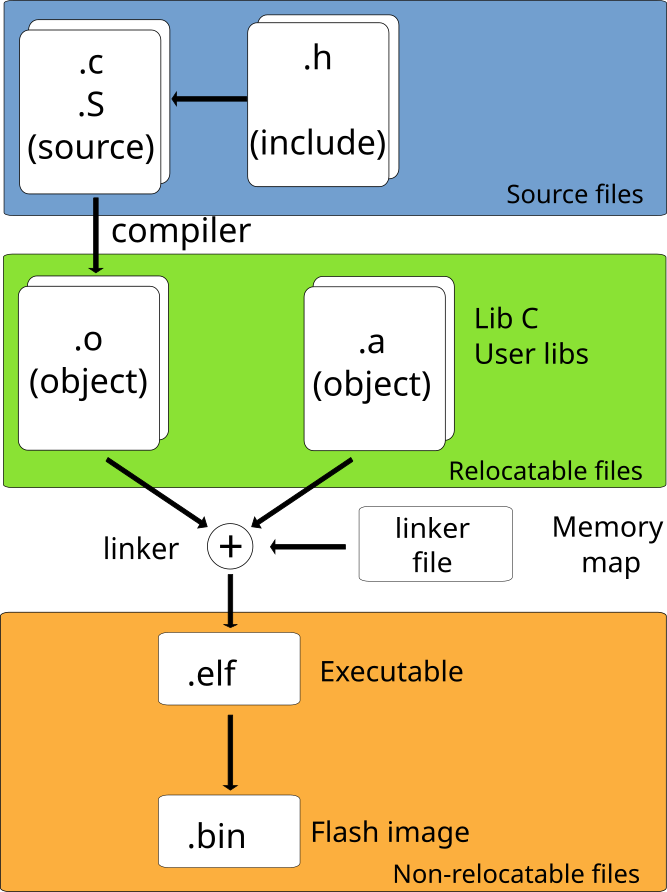
\includegraphics[scale=0.6]{imgs/compile_process.png}
	\end{center}	
\end{frame}

\begin{frame}
	\frametitle{Arquivos de inclusão}
	\begin{columns}[T] % align columns
		\begin{column}{.60\textwidth}
			\lstinputlisting[style=customc]{code/demo.h}
		\end{column}%
		\hfill%
		\begin{column}{.40\textwidth}
			\begin{itemize}
				\item Pense como API: só exporte interfaces e o que elas precisarem !
				\item Não esqueça a proteção de inclusão recursiva !				
				\item Não é ANSI-C mas \texttt{\textcolor{blue}{\#pragma once}} pode ser interessante
				\item Evite incluir arquivos de inclusão como boa prática
			\end{itemize}
		\end{column}%
	\end{columns}
\end{frame}

\begin{frame}
	\frametitle{Arquivos de inclusão}
	\lstinputlisting[style=customc]{code/accel.h}
\end{frame}

\begin{frame}
	\frametitle{Arquivos de código fonte}
	\begin{columns}[T] % align columns
		\begin{column}{.60\textwidth}
			\lstinputlisting[style=customc]{code/demo.c}
		\end{column}%
		\hfill%
		\begin{column}{.40\textwidth}
			\begin{itemize}
				\item Externe via funções o acesso a seus dados internos (encapsulamento)
				\item Dê escopo de arquivo para as suas funções e variáveis com static !
				\item Salve RAM colocando como const o que for realmente constante.
			\end{itemize}
		\end{column}%
	\end{columns}
\end{frame}

\begin{frame}
	\frametitle{Arquivos de código fonte}
	\lstinputlisting[style=customc]{code/accel.c}
\end{frame}


\begin{frame}[fragile]
	\begin{lstlisting}[style=customc]
		// test
		#include <stdio.h>
		int main(void)
		{
			printf("Hello World!"); 
		}
	\end{lstlisting}
\end{frame}

\begin{frame}
	\frametitle{Palavras Reservadas}
	\begin{itemize}
		\item x
	\end{itemize}	
\end{frame}


\end{document}